% Intended LaTeX compiler: pdflatex
\documentclass[10pt,a4paper,UTF8]{article}
\usepackage{zclorg}
\usepackage{tikztheorem}
\author{emacsun}
\date{}
\title{Git submodule 使用技巧}
\hypersetup{
 pdfauthor={emacsun},
 pdftitle={Git submodule 使用技巧},
 pdfkeywords={},
 pdfsubject={},
 pdfcreator={Emacs 25.2.1 (Org mode 9.0.9)},
 pdflang={English}}
\begin{document}

\maketitle
\tableofcontents
\titlepic{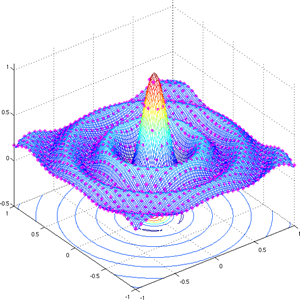
\includegraphics[scale=0.25]{../../img/sinc.PNG}}

\section{简介}
\label{sec:orga7ab815}

在工程 A 中有时候需要用到模块 b。而模块 b 是一个相对独立的模块,由别人维护,我们只需要定期更新模块 b 就可以了。如果把模块 b 也作为工程版本控制的一部分显然很麻烦,因为每次都从别人那里更新过来,再在当前工程下提交。git submodule 命令完美解决了这个问题。
\section{添加 submodule}
\label{sec:orgcbdfa3f}


第一次接触 git submodule 是通过 \href{http://gohugo.io/}{Hugo} 的一个主题 \href{https://themes.gohugo.io/docdock/}{docdock} 。通常,在 Hugo 根目录下会有一个 theme 文件夹。这里放置了静态博客使用的主题,这些主题在 github 上有自己的仓库。而我的博客也有自己的仓库。一种使用主题的方法是把主题 .zip 包下载下来,放到 hugo 根目录,同博客一起更新管理。但是这样就容易漏掉了主题所在的 github 上仓库的更新。并且主题的 github 仓库更新时,我还是要下载 .zip 包,并在我的仓库里提交这个主题的更新。 为了方便 theme 中的主题同 github 上主题同步,可以选择使用 git submodule.

具体操作为:
\begin{enumerate}
\item 在 hugo 根目录下添加 submodule
\end{enumerate}
\begin{verbatim}
$ git submodule add https://github.com/vjeantet/hugo-theme-docdock.git themes/docdock
\end{verbatim}
这时会在根目录下生成一个 \texttt{.gitmodules} 文件。
\begin{enumerate}
\item submodule 有更新时,只需要
\end{enumerate}
\begin{verbatim}
$ git submodule init
$ git submodule update
\end{verbatim}
即可更新 submodule.

\section{删除 submodule}
\label{sec:org8853986}


删除 submodule 的步骤:
\begin{enumerate}
\item 删除 \texttt{.gitmodules} 文件。
\item 执行 \texttt{git rm -cached} 把子模块从 git 中删除。
\end{enumerate}
\section{针对多个 submodule 的操作}
\label{sec:org84d50ae}

见\href{http://blog.csdn.net/wangjia55/article/details/24400501}{这里}

\section{参考}
\label{sec:org41185a7}

\begin{enumerate}
\item \href{http://blog.csdn.net/wangjia55/article/details/24400501}{git submodule 的使用}
\item \href{http://blog.csdn.net/wangjia55/article/details/24400501}{Hugo 主题 docdock}
\end{enumerate}
\end{document}
